\chapter{Machine Learning}\label{Machine Learning}

Machine learning is een welgekend begrip in de informatica wereld, maar wat het juist omvat, welke algmene technieken er bestaan en met welke factoren men moet rekening houden, wordt besproken in dit hoofdstuk.

\section{Wat is Machine Learning}\label{Wat is Machine Learning}

Over Machine Learnig vindt men nergens een eenduidige definitie. Vele hebben geprobeerd om een eenduidige definitie te definieren. Arthur Samuel(1959) definieerde machine learning als ``'Field of study that gives computers the ability to learn without being explicitly programmed''. Later stelde Tom Michel(1999) een well-posed learning problem als ``A computer program is said to learn from experience E with respect to some class of tasks T and performance measure P, if its performance at tasks in T, as measured by P, improves with experience E.'' Als men machine learnig wil omvatten, kan men het best omschrijven als een onderzoeksdomein dat zich bezighoudt met het onderzoeken en de ontwikkeling van zelflerende algoritmes.Hoofdzakelijk bestaat machine learning uit drie stappen namelijk data verzamelen, verwerken en analyseren.
\newline
Binnen machine learning kan men verschillende groepen van lerende algoritmes onderscheiden. Zo heeft men supervised learning, unsupervised learning, reinforcement learning en recommender systems. In deze voorbereiding gaat men zich enkel opleggen op supervised en unsupervised learning. Deze soorten algoritmen omvatten specifiekere technieken die zich lenen tot het gebruik bij text mining.


\section{Supervised Learning}\label{Supervised Learning}

Wanneer men een algoritme wil trainen, heeft men informatie nodig om het algoritme te trainen. Dergelijke informatie noemt men de trainingset.
\newline
Laat men als voorbeeld een trainingsset met positieve en negatieve artikels nemen. Men weet welke artikels positief en negatief zijn en ieder artikel bevat deze kennis aan de hand van een label. Het algoritme kan de informatie van de labels gebruiken om een zeker kennis te vergaren over artikels in het algemeen. Na het doorlopen van de trainingset, kan het algoritme de vergarde kennis gebruiken om een ongelabelde artikel te situeren als een positief of negatief artikel.
\newline
Deze techniek waarbij men een algoritme traint met een data waarvan men de antwoorden al weet noemt men supervised learning.
\newline
Het zelfstandig beslissingen maken over ongekende data is niet altijd even gemakkelijk en kan voor problemen zorgen. 
Bij supervised learning zijn er twee soorten problemen die kunnen optreden: een regressie probleem of een classification problem.

\subsection{Regressie Probleem}\label{Regressie Probleem}

Het doel dat men wil bereiken met supervised learning is dat het algoritme na een training antwoorden kan bezorgen over ongekende data. Bij het voorspellen van die antwoorden kan men te maken hebben met een regressie probleem. Dit probleem valt het best uit te leggen aan de hand van een voorbeeld. Neem nu dat men de prijs van een huis wilt voorspellen.
Het algoritme traint zich met een trainigset en bekomt volgend resultaat als men zijn bevindingen zou plotten.
\newline

%%TEKENENING HIER EEN GRAFIEK MET DATAPUNTEN 
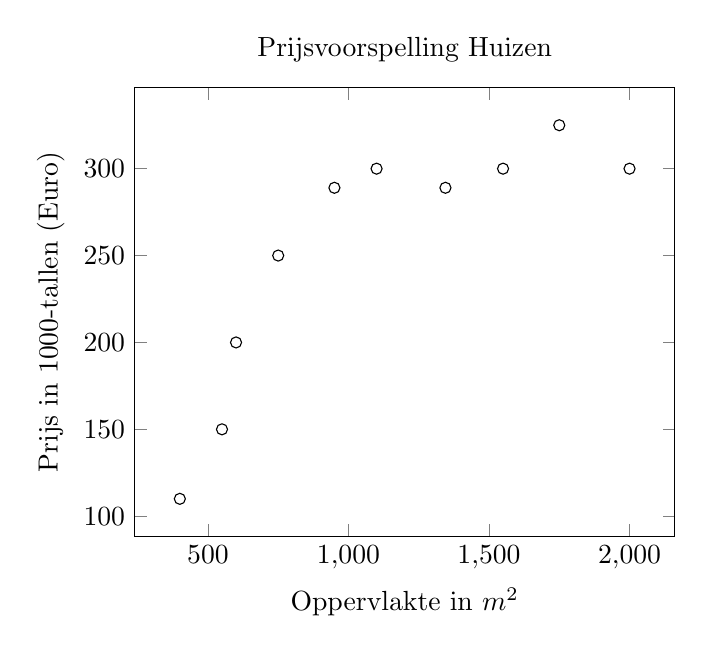
\begin{tikzpicture}
\begin{axis}[%
xlabel={Oppervlakte in $m^2$},
ylabel={Prijs in 1000-tallen (Euro)},
title={Prijsvoorspelling Huizen},
scatter/classes={%
    a={mark=o,draw=black}}]
\addplot[scatter,only marks,%
    scatter src=explicit symbolic]%
table[meta=label] {
x y label
400 110 a
550 150 a
600 200 a
750 250 a
950 289 a
1345 289 a
1550 300 a
1750 325 a
2000 300 a
1100 300 a
    };
\end{axis}
\end{tikzpicture}
\newline
Stel nu dat men aan het algoritme de prijs van een huis met 1225 vierkante meter vraagt. Deze waarde zat niet in de dataset en moet dus voorspeld worden. Maar welke trend moet men volgen om de waarden te voorspellen. Men kan zowel kiezen voor een rechte of een 2de orde polynoom. Beiden zijn een mogelijkheid, maar geven een verschillend antwoord. De situatie, waarbij men een continue waarde moet bepalen en geen echte discrete afbakening bestaat, noemt men een regressie probleem.
\newline
Om dit probleem op te lossen, kan men van de techniek \textbf{\textit{lineaire regressie}} gebruik maken.

\subsubsection{Lineaire regressie}\label{lineaire regressie}

Lineaire regressie is een techniek waarbij het algoritme een hypothese probeert te vormen. De hypothese is een functie die opgesteld is aan de hand van de trainigsset en de gekende en ongekende outputwaarden zo goed mogelijk benaderd.
\newline
Als we terug kijken naar het voorbeeld van het huis. Kan het algoritme volgende hypothese opstellen.

%%FORMULE VAN HYPOTHESE / IS EEN RECHTE MET 1 VARIABLE H(x) = %THETA1 X + THETA 0
\[H_{\theta}(x) = \theta_{0} + \theta_{1}x \]
Gegeven hypothese is een lineaire functie met als parameters $\theta_{0}$ de nulconditie en $\theta_{1}$ de richtingscoefficient. Een hypothese met \'e\'en functie noemt men ook wel een \'e\'endimensionale lineaire regressie.
\newline
Het opstellen van de hypothese introduceert op zijn beurt een \textbf{\textit{minimalisatie probleem}}. Men moet de hypothese zo goed mogelijk opstellen, zodat de afwijking ten op zichte van de gekende resultaten minimaal is. Als de hypothese minimaal is, kan men er van uit gaan dat de afwijking op ongekende resultaten ook minimaal is.
\newline
Het minimalisatie probleem kan opgelost worden met een \textbf{\textit{kost functie}} en \textbf{\textit{graduele afdaling}}.

\subsubsection{Kost Functie en Graduele afdaling}\label{Kost Functie en Gradule afdaling}

Men herneemt het voorbeeld van de prijsvoorspelling van huizen. Men moest een zo precies mogelijke prijs voorspellen voor een oppervlakte van 1225 $m^2$. Om dit probleem op te lossen gaat het algoritme gaat voor zowel rechten als 2de orde polynomen de kostfuncties berekenen. Dit gebeurd door de prijzen van de gekende oppervlaktes te vergelijken met de prijzen van de hypothese. Door telkens het verschil in prijs voor een bepaalde oppervlakte te nemen, deze op te tellen en het gemiddelde te nemen, verkrijgt men de gemiddelde afwijking van de prijs van de hypothese ten op zichte van de echte prijs. Hierdoor krijgt men een beeld over hoe de prijzen van de hypothese zich verhouden tegenover de eigelijke prijzen. De kost functie voor dit voorbeeld is  de functie met als functiewaarden de gemiddelde afwijkingen voor telkense een andere hypothese. Om dan een zo precies mogelijke voorspelling te kunnen doen voor de oppervlakte van 1225 $m^2$ moet men er voor zorgen dat men een hypothese kiest waarbij de gemiddelde afwijking zo laag mogelijk is.
\newline
Algemeen kan men de kost functie definieren als  een functie die voor een bepaalde waarden van de parameters de gemiddelde afwijking van de hypothese ten opzichten van de resultaten gaat berekenen.
\newline
Volgende formule kan men opstellen voor de kost functie:

%%FORMULE DE KOST FUNCTIE
\[J(\theta_{0},\theta_{1}) = \frac{1}{2m}\sum_{i=1}^{m} (H_{\theta}(x_i) - Y_i )^2\]
Deze kost functie noemt men ook wel de \textbf{\textit{squared error cost function}} en wordt over het algemeen het meest gebruikt. Merk op dat men niet zomaar telkens de som van het verschil tussen het resultaat van de hypothese neemt en de eigelijke waarden. Het kwadraat van het verschil wordt genomen vanwege de negatieve verschillen die ook moeten worden opgenomen als afwijking. Verder vereenvoudigt men het rekenwerk door te delen door twee (De helft van de kleinste waarde, blijft de kleinste waarde). 
\newline
Zoals eerder gezegd is het de bedoeling om de afwijking zo klein mogelijk te houden. Om het minimum van de kost functie te vinden, kan men de techniek \textbf{\textit{graduele afdeling}} gebruiken. Omwille van verschillende redenen is graduele afdaling een van de meest gebruikte techniek binnen machine learning voor minimalisatie. Zo werkt de techniek voor een algemeen kost functie met n parameters J($\theta_{0},\theta_{1},\theta_{2},\theta_{3}, ... ,\theta_{n}$) en kan het altijd uitgevoert worden aangezien de lineaire regressie kost functie altijd convex is.
\newline
De techniek start met een random start punt te nemen. Vervolgens gaat men stapsgewijs proberen te dalen tot je convergeert naar een lokaal minimum.
\newline
De preciese werking van het algoritme valt het best uit te leggen aan de hand van een voorbeeld. We nemen als voorbeeld onze eerder opgestelde hypothese met twee parameters $\theta_{0}$ en $\theta_{1}$. Als men de kost functie J($\theta_{0}, \theta_{1}$) berekent en deze weergeeft in een driedimensionale weergave, krijgt men onderstaande plot.
%AFBEELDING VAN EEN 3D-PLOT
%beschrijving: van axissen
\begin{center}
  \includegraphics[width=10cm]{3d_plot}
  \captionof{figure}{Driedimensionale weergave van de kostfunctie en zijn parameters}
\end{center}
%
Het stapgewijs dalen kan als volgende formeel neergeschreven worden:

%%FORMULE STAPGEWIJS DALEN
\[ \theta_{j} := \theta_{j} - \alpha\frac{d}{d\theta_{j}}J(\theta_{0},\theta_{1})   \text{  (voor j = 0 en j = 1)}\] 
Alfa noemt men hier de learning rate. Dit is de grote van de stappen die men neemt bij het afdalen. De learning rate is een belangrijk element in het graduele afdalingsalgoritme. Als men deze te groot neemt kan men locale minima overslagen en convergeert het algoritme niet. Als men alfa te klein neemt kan het algoritme heel lang duren. 
\newline
Een belangrijk en subtiel detail bij de formule en het algoritme is het simultaan updaten van de twee parameters (zowel $\theta_{0}$ als $\theta_{1}$). Als men dit niet doet, spreekt men niet van graduele afdaling.
\newline
Een bedenking die men moet maken bij graduele afdaling is het bestaan van meerdere lokale minima. Dit kan men echter eenvoudig oplossen door meerdere keren het algoritme uit te voeren met een ander startpunt.
\newline
Het gegeven voorbeeld noemt men specifieker \textbf{\textit{batch graduele afdaling}} waarbij men telkens bij iedere stap de hele trainingsset vergelijkt. Er bestaan ook niet batch versies van graduele afdaling.

\subsection{Classificatie Probleem}\label{Classificatie Probleem}

Een classificatie probleem is een ander soort van probleem dat zich voordoet bij supervised training. Een classificatie probleem doet zich voor wanneer men data moeten verdelen over verschillende discrete klassen en reder elemenent maar tot \'e\'en klasse mag behoren. De classificatie kan gebaseerd zijn op \'e\'en attribuut, maar ook op meerdere.
\newline
In het algemeen wordt het classificatie probleem het meest opgelost door \textbf{\textit{logistische regressie}}    

\section{Unsupervised Learning}\label{Unsupervised Learning}

Unsupervised learning is een techniek waarbij het algoritme zelfstandig moet leren hoe het juist moet en deze kennis gebruikt om later patronen en structuren in data te herkennen. De trainingsset bevat niet de antwoorden.
\newline
Als men het zou vergelijken met het voorbeeld van supervised learning, zou men bij unsupervised learning als voorbeeld de situatie kunnen nemen waarbij het algoritme een ongelabelde trainingsset van artikels krijgt en na het verwerken van deze artikels zelfstandig keuzes kan maken over welke artikels positief en negatief zijn.
\newline
Echter kan een algoritme de structuren en patronen herkennen, maar kan het niet de data concreet identificeren. Dit probleem kan men oplossen door gebruik te maken van cluster algoritmes. Concreet gaat een cluster algoritme de data groeperen of \textbf{\textit{clusteren}} in groepen en zo de data concreet identificeren.



